\section{例题与分析}

\begin{question}\begin{example}[小球放入空腔的接触与未接触]\label{e3:example:1}
带正电 $q$ 的小球放入原中性的闭合金属空腔。分别讨论保持绝缘、不接触腔壁，以及接触后再分离两种过程的内外表面总电荷。
\end{example}
\typeout{ECFIG:fig:e3:example:1:s}\fig{fig:e3:example:1:s}{题设：小球放入空腔的接触与未接触}{\begin{tikzpicture}[scale=.88]
\fill[gray!18](0,0)circle(1.8);\fill[white](0,0)circle(1.3);\draw[world](0,0)circle(1.8);\draw[world](0,0)circle(1.3);\node at(2.8,1.5){金属};\draw[world,fill=white](0.4,0.1)circle(.12);\node[above]at(0.4,0.25){$q$};
\end{tikzpicture}}
\end{question}
\begin{solution}\textbf{未接触时先用金属内的高斯面定内壁总量}\par\nobreak
图\ref{fig:e3:example:1:s} 未接触时，在金属中取包围腔的高斯面，由内部场零得 $q+Q_{\text{内}}=0$，所以内表面总量 $-q$。壳仍中性，故外表面总量 $+q$。
\typeout{ECFIG:fig:e3:example:1:p}\fig{fig:e3:example:1:p}{未接触时内外感应相反；接触达到平衡后，净量只在最外表面，腔内小球分离后无净量}{\begin{tikzpicture}
\begin{scope}[scale=.85]\fill[gray!12](0,0)circle(1.6);\fill[white](0,0)circle(1.1);\draw(0,0)circle(1.6);\draw(0,0)circle(1.1);
\fill(.3,.1)circle(2pt)node[above]{$+q$};\draw[guide](0,0)circle(1.35);\node at(-.45,-.5){内 $-q$};\node at(0,2.3){未接触};\node at(0,-2.2){外 $+q$};
\end{scope}\begin{scope}[xshift=4.7cm,scale=.85]\fill[gray!12](0,0)circle(1.6);\fill[white](0,0)circle(1.1);\draw(0,0)circle(1.6);\draw(0,0)circle(1.1);
\draw(.85,0)circle(.25);\draw[thick](.9,0)--(1.15,0);\node at(0,2.3){接触后平衡};\node at(-.2,-.4){内 $0$};\node at(0,-2.2){外 $+q$};
\end{scope}\begin{scope}[xshift=9.4cm,scale=.85]\fill[gray!12](0,0)circle(1.6);\fill[white](0,0)circle(1.1);\draw(0,0)circle(1.6);\draw(0,0)circle(1.1);
\draw(.2,0)circle(.2);\node at(-.3,.5){小球 $0$};\node at(-.25,-.5){内 $0$};\node at(0,2.3){再分离};\node at(0,-2.2){外 $+q$};
\end{scope}

\end{tikzpicture}}



\par\medskip\Needspace{4\baselineskip}\noindent\textbf{接触后按一个连通体求静电平衡}\par\nobreak
图\ref{fig:e3:example:1:p} 接触后小球与壳连通，腔内没有独立的自由电荷，连通体内部腔壁为同电势，空腔零场；净 $+q$ 全在最外表面。

\par\medskip\Needspace{4\baselineskip}\noindent\textbf{分离时保留小球的零净量并比较两种过程}\par\nobreak
若小球完全位于腔内并在平衡后分离，它原来所处的内表面没有净电荷，分离后保持零净量。两种过程分别对应“内负外正”和“仅外表面带正电”，不能省略是否接触这一条件。\end{solution}
\begin{question}\begin{example}[先后触碰两个导体的净电荷]\label{e3:example:2}
正电小球 $C$ 固定在空腔导体 $A$ 内而不接触。外部另有中性导体 $B$。先短暂接地 $A$ 后撤去地线，再短暂接地 $B$ 后撤线，最后移走 $C$。判断 $A,B$ 的最终净电荷，忽略小孔漏场。
\end{example}
\typeout{ECFIG:fig:e3:example:2:s}\fig{fig:e3:example:2:s}{题设：先后触碰两个导体的净电荷}{\begin{tikzpicture}[scale=.88]
\fill[gray!18](0,0)circle(1.8);\fill[white](0,0)circle(1.3);\draw[world](0,0)circle(1.8);\draw[world](0,0)circle(1.3);\node at(2.8,1.5){金属};\draw[world,fill=white](0,0)circle(.12);\node[above]at(0,0.15){$C:+q$};\node at(0,2.3){$A$};\draw[world](4,0)circle(.5);\node at(4,0){$B$};
\end{tikzpicture}}
\end{question}
\begin{solution}\textbf{接地空腔导体后再撤线，固定所得净量}\par\nobreak
图\ref{fig:e3:example:2:s} 首先接地 $A$ 时，内表面感应 $-q$，外部没有其他电荷，接地外区域的零势解使外表面为零，故 $A$ 净量为 $-q$。撤地后这一净量保持。



\par\medskip\Needspace{4\baselineskip}\noindent\textbf{用外部零场判断第二个导体的接地结果}\par\nobreak
接地 $B$ 的阶段，$C$ 与 $A$ 内表面总量相消，外表面仍为零，外区域没有由这组内部电荷产生的场，所以 $B$ 无须取得净电荷，仍为零。
\typeout{ECFIG:fig:e3:example:2:p}\fig{fig:e3:example:2:p}{按地线状态逐阶段记录；撤线后的净量固定，最后移走内电荷只引起重新分布}{\begin{tikzpicture}
\begin{scope}[scale=.8]\fill[gray!12](0,0)circle(1.6);\fill[white](0,0)circle(1.1);\draw(0,0)circle(1.6);\draw(0,0)circle(1.1);
\fill(0,0)circle(2pt)node[above]{$C:+q$};\draw(0,-1.6)--(0,-2.5)node[ground]{};\draw(3.2,0)circle(.45);\node at(3.2,0){$B$};
\node at(0,2.2){$A$ 接地};\node at(0,-3.6){$Q_A=-q$};
\end{scope}\begin{scope}[xshift=4.8cm,scale=.8]\fill[gray!12](0,0)circle(1.6);\fill[white](0,0)circle(1.1);\draw(0,0)circle(1.6);\draw(0,0)circle(1.1);
\fill(0,0)circle(2pt)node[above]{$C:+q$};\draw(3.2,0)circle(.45);\node at(3.2,0){$B$};\draw(3.2,-.45)--(3.2,-2.5)node[ground]{};
\node at(0,2.2){$A$ 撤线，$B$ 接地};\node at(0,-3.6){$Q_A=-q,\ Q_B=0$};
\end{scope}\begin{scope}[xshift=9.6cm,scale=.8]\fill[gray!12](0,0)circle(1.6);\fill[white](0,0)circle(1.1);\draw(0,0)circle(1.6);\draw(0,0)circle(1.1);
\draw(3.2,0)circle(.45);\node at(3.2,0){$B$};\node at(0,0){无 $C$};\node at(0,2.2){两者撤线后移走 $C$};\node at(0,-3.6){净量仍为 $-q,0$};
\end{scope}

\end{tikzpicture}}



\par\medskip\Needspace{4\baselineskip}\noindent\textbf{说明外部零场依靠完整边界条件}\par\nobreak
这里第二次接地时，$A$ 外部零场由完整边界解保证，不只是“包围净量零”的推测：外表面可取零势、外部无其他源，唯一性给出外部零场。$B$ 此时原中性且不受外场，接地不会改变其零净量。



\par\medskip\Needspace{4\baselineskip}\noindent\textbf{两者孤立后只重排，不再改变净量}\par\nobreak
图\ref{fig:e3:example:2:p} 最后移走 $C$ 时，$A$ 已孤立，保持净量 $-q$，它重新分布到最外表面；$B$ 也已孤立，净量仍为零，但可在 $A$ 的外场下出现局部正负感应。应答为 $A$ 带负净电、$B$ 无净电，不能把“无净电”写成“表面处处没有电荷”。\end{solution}
\begin{question}\begin{example}[外部带电球靠近屏蔽腔]\label{e3:example:3}
正电小球 $A$ 悬于中性闭合球壳 $C$ 的球心，另一悬挂负电小球 $B$ 从外靠近。壳固定且不接地，忽略穿线孔。判断 $A$ 是否发生新的水平偏转、$B$ 是否被吸向壳。
\end{example}
\typeout{ECFIG:fig:e3:example:3:s}\fig{fig:e3:example:3:s}{题设：外部带电球靠近屏蔽腔}{\begin{tikzpicture}[scale=.88]
\fill[gray!18](0,0)circle(1.8);\fill[white](0,0)circle(1.3);\draw[world](0,0)circle(1.8);\draw[world](0,0)circle(1.3);\node at(2.8,1.5){金属};\draw[world,fill=white](0,0)circle(.12);\node[above]at(0,0.15){$A:+q$};\draw[world,fill=white](-3.5,0)circle(.12);\node[above]at(-3.5,0.15){$B:-q_B$};\draw(0,.15)--(0,2.7)(-3.5,.15)--(-3.5,2.7);\draw[world](-4,2.7)--(.5,2.7);
\end{tikzpicture}}
\end{question}
\begin{solution}\textbf{用封闭腔的边界判断内部电荷是否偏转}\par\nobreak
图\ref{fig:e3:example:3:s} 腔壁电势可因外部小球靠近而整体改变，但腔内由原电荷造成的场不变。原 $A$ 在球心时内表面对称，水平合力为零，外部 $B$ 不能透过理想闭腔使 $A$ 出现新的水平偏转。
\typeout{ECFIG:fig:e3:example:3:p}\fig{fig:e3:example:3:p}{内壁的球对称感应使中心电荷无水平合力；外部负电荷仍受吸引}{\begin{tikzpicture}

\fill[gray!12](0,0)circle(1.8);\fill[white](0,0)circle(1.25);\draw(0,0)circle(1.8);\draw(0,0)circle(1.25);
\draw(0,0)--(0,2.7);\fill(0,0)circle(2pt)node[right]{$A$};\node at(0,-.7){$F_{Ax}=0$};
\fill(-3.8,0)circle(2pt)node[above]{$B<0$};\draw[force](-3.8,0)--(-2.4,0)node[midway,below]{$F_B$};
\draw[guide](-1.1,.6)--(-2.6,1.7)node[above]{内壁总量 $-q$};\draw[guide](1.5,.8)--(3,1.6)node[right]{外表面总量 $+q$};

\end{tikzpicture}}



\par\medskip\Needspace{4\baselineskip}\noindent\textbf{按外表面净量和极化判断外部吸引}\par\nobreak
图\ref{fig:e3:example:3:p} 壳内表面总量 $-q$，外表面总量 $+q$，所以壳没有屏蔽内部净电荷对外的全部影响。负电 $B$ 受到外部正电及近侧感应作用吸引，偏向壳。

\par\medskip\Needspace{4\baselineskip}\noindent\textbf{区分屏蔽腔内场与消除外部相互作用}\par\nobreak
结论是 $A$ 不变、$B$ 向壳；若壳接地且外侧只剩 $B$ 自身，$B$ 仍会因自身诱导的像电荷而被吸引，不能把接地屏蔽解释为消除所有外部相互作用。\end{solution}
\begin{question}\begin{example}[带罩验电器的三阶段变化]\label{e3:example:4}
验电器的小球 $A$、金属杆 $B$ 与金箔 $C$ 相连，与金属罩 $D$ 绝缘。整体置绝缘座上。给 $A$ 正电；再用绝缘柄金属叉连接 $A,D$；撤叉后用手触 $A$。判断各阶段金箔变化，忽略小穿线孔漏场。
\end{example}
\typeout{ECFIG:fig:e3:example:4:s}\fig{fig:e3:example:4:s}{金属杆穿过绝缘塞，与罩 $D$ 不接触；图示给电前的结构}{\begin{tikzpicture}

\draw(0,0)circle(1.7);\fill[white](-.2,1.4)rectangle(.2,2);\draw(-.2,1.4)rectangle(.2,2);
\draw(0,2.7)circle(.2);\draw(0,2.5)--(0,-.2);\draw(-.04,-.2)--(-.04,-.95)(.04,-.2)--(.04,-.95);
\node[right]at(.2,2.7){$A$};\node[right]at(0,.6){$B$};\node[right]at(.3,-.8){$C$};\node[right]at(1.7,.8){$D$};
\draw[guide](.2,1.7)--(2.3,2)node[right]{绝缘塞};\node at(0,-2.3){绝缘座};

\end{tikzpicture}}
\end{question}
\begin{solution}\textbf{给内电极正电时金箔同号排斥}\par\nobreak
在 图\ref{fig:e3:example:4:s} 第一步，正电进入小球—杆—金箔的连通体，两片金箔带同号电，张开。金属罩可感应，但它与杆尚不等势，不能把内部金箔的电荷全部转走。
\typeout{ECFIG:fig:e3:example:4:p}\fig{fig:e3:example:4:p}{左图正电金箔张开；中图金属叉把内外连通，金箔闭合；右图撤叉后内电极接地，金箔带负电再张开}{\begin{tikzpicture}
\begin{scope}[scale=.8]\draw(0,0)circle(1.6);\fill[white](-.2,1.3)rectangle(.2,1.9);\draw(-.2,1.3)rectangle(.2,1.9);\draw(0,2.6)circle(.18);\draw(0,2.42)--(0,-.15);\draw(0,-.15)--(-.55,-.9)(0,-.15)--(.55,-.9);\node at(-.65,-.5){$+$};\node at(.65,-.5){$+$};\node at(0,-2.4){给 $A$ 正电};\end{scope}\begin{scope}[xshift=4.5cm,scale=.8]\draw(0,0)circle(1.6);\fill[white](-.2,1.3)rectangle(.2,1.9);\draw(-.2,1.3)rectangle(.2,1.9);\draw(0,2.6)circle(.18);\draw(0,2.42)--(0,-.15);\draw(-.06,-.15)--(-.06,-.9)(.06,-.15)--(.06,-.9);\draw[blue,thick](.18,2.6)--(1.7,2.6)--(1.7,.5)--(1.52,.5);\node at(-1.3,.6){$+$};\node at(1.3,-.6){$+$};\node at(0,-2.4){$A,D$ 连通};\end{scope}\begin{scope}[xshift=9cm,scale=.8]\draw(0,0)circle(1.6);\fill[white](-.2,1.3)rectangle(.2,1.9);\draw(-.2,1.3)rectangle(.2,1.9);\draw(0,2.6)circle(.18);\draw(0,2.42)--(0,-.15);\draw(0,-.15)--(-.55,-.9)(0,-.15)--(.55,-.9);\draw(0,2.78)--(0,3.4)--(-1.8,3.4)--(-1.8,2.5)node[ground]{};\node at(-.65,-.5){$-$};\node at(.65,-.5){$-$};\node at(-1.3,.6){$+$};\node at(1.3,-.6){$+$};\node at(0,-2.4){撤叉后接地 $A$};\end{scope}
\end{tikzpicture}}



\par\medskip\Needspace{4\baselineskip}\noindent\textbf{金属叉连通内外后由同一导体等势求闭合}\par\nobreak
图\ref{fig:e3:example:4:p} 第二步连接 $A,D$，两者成为一个连通导体。静电平衡后内腔没有独立电荷，内腔场零，金箔上不保留同号排斥电荷，闭合；净正电分布于整个连通体的外表面。撤叉使两部分各保留分离时状态。



\par\medskip\Needspace{4\baselineskip}\noindent\textbf{撤叉后接地内电极，重新建立感应负电}\par\nobreak
最后手触 $A$ 使杆和金箔接地，外罩仍孤立并带正电，内部接地电极与外罩不再等势。外罩正电使内电极感应负电，金箔再次带同号负电，张开。

\par\medskip\Needspace{4\baselineskip}\noindent\textbf{核对三阶段的张合与电荷符号}\par\nobreak
因此变化依次为张开、闭合、再张开。不能因两次金箔都张开就认定两次带电符号相同。\end{solution}
\begin{question}\begin{example}[远隔两球连线后的分配]\label{e3:example:5}
两金属球半径 $R_1,R_2$，相距远大于两半径，用细导线连接，总电量 $Q$。忽略导线电荷和相互电势，求电量、面密度、表面场之比与共同电势。
\end{example}
\typeout{ECFIG:fig:e3:example:5:s}\fig{fig:e3:example:5:s}{题设：远隔两球连线后的分配}{\begin{tikzpicture}[scale=.88]
\draw[world](0,0)circle(1.2);\draw[world](5,0)circle(.6);\draw[world](1.2,0)--(4.4,0);\node at(0,0){$R_1$};\node at(5,0){$R_2$};\node at(2.7,.7){细导线，远隔};
\end{tikzpicture}}
\end{question}
\begin{solution}\textbf{用等势与总量守恒联立求电荷分配}\par\nobreak
图\ref{fig:e3:example:5:s} 连接后电势相同，$Q_1/R_1=Q_2/R_2$，总量 $Q_1+Q_2=Q$。联立得 $Q_i=QR_i/(R_1+R_2)$，共同电势 $V=kQ/(R_1+R_2)$。
\typeout{ECFIG:fig:e3:example:5:p}\fig{fig:e3:example:5:p}{共同电势下以 $R_1=2R_2$ 示意；场箭头长度按正电情况下的 $E_2=2E_1$ 绘制}{\begin{tikzpicture}

\draw(0,0)circle(1.5);\draw(6,0)circle(.75);\draw(1.5,0)--(5.25,0);\node at(0,0){$Q_1,R_1$};\node at(6,0){$Q_2,R_2$};
\draw[flow](0,1.5)--(0,2.3)node[above]{$E_1$};\draw[flow](6,.75)--(6,2.35)node[above]{$E_2$};
\node at(3,-2){$V_1=V_2=kQ/(R_1+R_2)$};

\end{tikzpicture}}



\par\medskip\Needspace{4\baselineskip}\noindent\textbf{再按表面积换算面密度和表面场}\par\nobreak
图\ref{fig:e3:example:5:p} 每球面密度 $\sigma_i=Q_i/(4\pi R_i^2)$，故 $Q_1:Q_2=R_1:R_2$，$\sigma_1:\sigma_2=R_2:R_1$，表面场大小比同为 $R_2:R_1$。

\par\medskip\Needspace{4\baselineskip}\noindent\textbf{检查半径比模型的远隔条件}\par\nobreak
小球分得的总电荷较少，局部面密度和表面场却较大。若两球靠近，相互极化和电势贡献不能忽略，这些简单比值不再精确。\end{solution}
\begin{question}\begin{example}[同心小球与厚球壳]\label{e3:example:6}
半径 $r$ 的金属球与内外半径 $R_1,R_2$ 的金属壳同心，$r<R_1$。小球电量 $q$、壳净量 $Q$，无外部电荷。求小球电势、两壳面的电量及两导体电势差；再将壳接地，重求。
\end{example}
\typeout{ECFIG:fig:e3:example:6:s}\fig{fig:e3:example:6:s}{同心几何中三个半径分开标记，壳净量为 $Q$，中央球净量为 $q$}{\begin{tikzpicture}

\fill[gray!12](0,0)circle(2.3);\fill[white](0,0)circle(1.7);\draw(0,0)circle(2.3);\draw(0,0)circle(1.7);\draw(0,0)circle(.65);\node at(0,.2){$q$};
\draw[<->](0,0)--(.65,0)node[midway,below]{$r$};\draw[<->](0,0)--(-1.2,1.2)node[midway,left]{$R_1$};\draw[<->](0,0)--(1.15,1.992)node[midway,right]{$R_2$};\node at(3.7,-.5){壳净量 $Q$};

\end{tikzpicture}}
\end{question}
\begin{solution}\textbf{按高斯面与球对称确定三个球面的电荷}\par\nobreak
图\ref{fig:e3:example:6:s} 中金属壳内高斯面给内表面 $-q$，外表面 $Q+q$；球对称使它们各自均匀。小球表面电势
\[
 V_{\text{球}}=k\left[\frac qr-\frac q{R_1}+\frac{Q+q}{R_2}\right],
\]
壳电势 $V_{\text{壳}}=k(Q+q)/R_2$，所以电势差 $kq(1/r-1/R_1)$。
\typeout{ECFIG:fig:e3:example:6:p}\fig{fig:e3:example:6:p}{接地只消去共同外部电势项；间隙仍由中心球电荷 $q$ 决定}{\begin{tikzpicture}

\fill[gray!12](0,0)circle(2.3);\fill[white](0,0)circle(1.7);\draw(0,0)circle(2.3);\draw(0,0)circle(1.7);\draw(0,0)circle(.65);\node at(0,0){$q$};
\draw(0,-2.3)--(0,-3.2)node[ground]{};\draw[guide](-1.5,.8)--(-3,1.6)node[left]{内面 $-q$};\draw[guide](2.1,.7)--(3,1.7)node[right]{外面 $0$};
\draw[flow](.8,0)--(1.55,0)node[midway,above]{$\bm E$};\node at(4,-.6){$V_{\text{壳}}=0$};

\end{tikzpicture}}



\par\medskip\Needspace{4\baselineskip}\noindent\textbf{沿真实间隙场独立核对球壳势差}\par\nobreak
也可直接沿径向间隙求差：
\[
V_{\text{球}}-V_{\text{壳}}=\int_r^{R_1}\frac{kq}{s^2}\dd s
=kq[-s^{-1}]_r^{R_1}
 =kq\left(\frac1r-\frac1{R_1}\right).
\]
积分路径从小球表面到壳内表面，金属厚度区无场，故差值与 $R_2$ 及外部共同电势无关。图\ref{fig:e3:example:6:p}的场箭头以 $q>0$ 为例。





\par\medskip\Needspace{4\baselineskip}\noindent\textbf{接地后重定外表面总量与共同电势}\par\nobreak
图\ref{fig:e3:example:6:p} 接地后壳电势零，外部无电荷使外表面电量为零，内表面仍为 $-q$，壳从大地取得净量 $-q$。小球电势变为 $kq(1/r-1/R_1)$，而球—壳电势差保持不变。

\par\medskip\Needspace{4\baselineskip}\noindent\textbf{比较接地前后不变的间隙场与势差}\par\nobreak
接地改变共同的外部电势项，不改变由间隙场决定的差值。内外壳面密度分别用各自电量除 $4\pi R_i^2$，不能都用外半径。\end{solution}
\begin{question}\begin{example}[点电荷与接地平面的场和功]\label{e3:example:7}
正电荷 $q$ 位于接地无限大导体平面右侧，距面 $d$。求右侧电场、金属内部感应电荷的场、表面面密度、总感应电荷、作用力，以及将 $q$ 缓慢移至无穷远的外力功。
\end{example}
\typeout{ECFIG:fig:e3:example:7:s}\fig{fig:e3:example:7:s}{题设：点电荷与接地平面的场和功}{\begin{tikzpicture}[scale=.88]
\fill[pattern=north east lines](-.45,-2)rectangle(0,2);\draw[world](0,-2)--(0,2);\node[ground]at(-.2,-2){};\draw[world,fill=white](2,0)circle(.12);\node[above]at(2,0.15){$q$};\draw[dim](0,-1.2)--(2,-1.2)node[midway,below]{$d$};
\end{tikzpicture}}
\end{question}
\begin{solution}\textbf{先用反号镜像满足平面零势边界}\par\nobreak
在 图\ref{fig:e3:example:7:s} 中以平面为 $x=0$，真电荷在 $x=d$。在真实求解区域之外、金属一侧，图\ref{fig:e3:example:7:p} 的像电荷 $-q$ 放在 $x=-d$，平面上到两电荷距离相同，两势相消，且无穷远势为零。因此真实右半空间的电势为
\[
 V(x,s)=kq\left[\frac1{\sqrt{(x-d)^2+s^2}}-\frac1{\sqrt{(x+d)^2+s^2}}\right],\quad x>0.
\]


\par\medskip\Needspace{4\baselineskip}\noindent\textbf{由电势分别求轴向和横向电场}\par\nobreak
令 $r_1=\sqrt{(x-d)^2+s^2}$、$r_2=\sqrt{(x+d)^2+s^2}$，先分别计算两个倒数距离的偏导。以第一项为例，
\[
 \partial_x(r_1^{-1})=-\frac12r_1^{-3}\,2(x-d)
 =-\frac{x-d}{r_1^3},\qquad
 \partial_s(r_1^{-1})=-\frac12r_1^{-3}\,2s=-\frac{s}{r_1^3}.
\]
第二项将 $x-d$ 换为 $x+d$。再用 $E_x=-\partial_xV$、
$E_s=-\partial_sV$，并保留电势中第二项的负号，
右侧电场的轴向、横向分量为
\[
E_x=kq\left(\frac{x-d}{r_1^3}-\frac{x+d}{r_2^3}\right),\qquad
E_s=kqs\left(\frac1{r_1^3}-\frac1{r_2^3}\right),\quad E_\varphi=0.
\]


\par\medskip\Needspace{4\baselineskip}\noindent\textbf{在金属内另用总场为零求感应场}\par\nobreak
金属内部真实总场为零，故那里感应电荷的场恰为真电荷场的反向；不能把右半空间的像公式直接当成金属内部的真实总场。
对金属内 $x<0$ 的点 $\bm r$，感应场应另写为
\[
\bm E_{\text{感}}(\bm r)=-kq\frac{\bm r-d\hat{\bm x}}{|\bm r-d\hat{\bm x}|^3}.
\]
该式由真实金属中 $\bm E_{\text{真点}}+\bm E_{\text{感}}=0$ 得到；不把像点当作金属内的真实奇点。

\typeout{ECFIG:fig:e3:example:7:p}\fig{fig:e3:example:7:p}{像在真实求解区之外；在导体表面 $P$ 作法向投影，切向分量抵消，电荷受力朝向平面}{\begin{tikzpicture}

\fill[gray!10](-3,-1.8)rectangle(0,2.4);\draw[thick](0,-1.8)--(0,2.4);\draw(0,-1.8)--(0,-2.6)node[ground]{};
\fill(2,0)circle(2pt)node[above]{$q$};\draw[blue,dashed](-2,0)circle(.12);\node[blue,above]at(-2,.2){$-q$};
\draw[force](2,-.4)--(.7,-.4)node[midway,below]{$F_x<0$};\fill(0,1.2)circle(2pt)node[right]{$P$};
\draw[guide](-2,0)--(0,1.2)--(2,0);\draw[flow,gray](0,1.2)--(-.8,.72);\draw[flow,gray](0,1.2)--(-.8,1.68);
\draw[flow,blue](0,1.2)--(-1.3,1.2);\node[fill=white]at(-1.4,2){真实金属 $E=0$};
\draw[<->](-2,-1.4)--(2,-1.4)node[midway,below]{$2d$};\node at(3.8,1.6){$x>0$};

\end{tikzpicture}}



\par\medskip\Needspace{4\baselineskip}\noindent\textbf{由法向场求面密度并积分总量}\par\nobreak
在表面取向右法向，$E_x(0^+,s)=-2kqd/(d^2+s^2)^{3/2}$，所以
\[
 \sigma(s)=-\frac{qd}{2\pi(d^2+s^2)^{3/2}},\qquad
 Q_g=\int_0^\infty \sigma(s)2\pi s\,\dd s
=-qd\int_0^\infty\frac{s\dd s}{(d^2+s^2)^{3/2}}.
\]
这里的原函数由 $u=d^2+s^2$、$\dd u=2s\dd s$ 得到：
\[
 \int_0^S\frac{s\dd s}{(d^2+s^2)^{3/2}}
 =\frac12\int_{d^2}^{d^2+S^2}u^{-3/2}\dd u
 =[-u^{-1/2}]_{d^2}^{d^2+S^2}
 =\frac1d-\frac1{\sqrt{d^2+S^2}}.
\]
取 $S\to\infty$ 后，再乘 $-qd$，即得总感应量
\[
 Q_g=-qd\left(\frac1d-0\right)=-q.
\]


\par\medskip\Needspace{4\baselineskip}\noindent\textbf{用真像间距求力并积分缓慢拉离功}\par\nobreak
真电荷受到的力由距它 $2d$ 的像计算，方向朝向平面，$F_x=-kq^2/(4d^2)$。从 $d$ 缓慢拉到无穷远，外力作功
\[
 W_{\text{外}}=\frac{kq^2}{4}\lim_{L\to\infty}
 \int_d^Lx^{-2}\dd x
 =\frac{kq^2}{4}\lim_{L\to\infty}[-x^{-1}]_d^L
 =\frac{kq^2}{4}\left(0+\frac1d\right)=\frac{kq^2}{4d}.
\]


\par\medskip\Needspace{4\baselineskip}\noindent\textbf{解释相互作用能中的二分之一}\par\nobreak
因而相互作用能为 $U=-kq^2/(4d)$，等于 $\tfrac12qV_{\text{感}}$。直接用 $qV_{\text{感}}=-kq^2/(2d)$ 会多一倍，因为诱导分布是在放入 $q$ 的同时逐渐建立的。\end{solution}
\begin{question}\begin{example}[接地金属球的像、力与拉离功]\label{e3:example:8}
半径 $R$ 的接地金属球，外点电荷 $q$ 在距球心 $d>R$ 处。求像电荷位置与大小、球面感应总量、对 $q$ 的力与缓慢拉离功。
\end{example}
\typeout{ECFIG:fig:e3:example:8:s}\fig{fig:e3:example:8:s}{球接地，外电荷距球心 $d>R$；球面半径与源点距离分别标明}{\begin{tikzpicture}
\draw(0,0)circle(1.8);\fill(0,0)circle(1.5pt)node[below]{$O$};\draw[<->](0,0)--(-1.273,1.273)node[midway,left]{$R$};\fill(4,0)circle(2pt)node[above]{$q$};\draw(0,-1.8)--(0,-2.8)node[ground]{};\draw[<->](0,-3.4)--(4,-3.4)node[midway,below]{$d$};
\end{tikzpicture}}
\end{question}
\begin{solution}\textbf{要求整个球面上真像距离保持固定比例}\par\nobreak
沿 图\ref{fig:e3:example:8:s} 的球心—电荷轴取像于球内距心 $b$ 处。球面点 $P$ 到真、像的距离分别为 $\ell,\ell^\prime$。要求两者比值在整个球面恒定，比较
\[
 \ell^2=d^2+R^2-2dR\cos\theta,\quad
 {\ell^\prime}^2=b^2+R^2-2bR\cos\theta
\]
的常数项和 $\cos\theta$ 项，可取 $b=R^2/d$，此时 $\ell^\prime=(R/d)\ell$。因此 $q^\prime=-qR/d$ 时，$q/\ell+q^\prime/\ell^\prime=0$，球面满足接地条件。
\typeout{ECFIG:fig:e3:example:8:p}\fig{fig:e3:example:8:p}{球面所有点都满足距离比；力由真像间距 $d-b$ 决定，像位于球内}{\begin{tikzpicture}
\draw(0,0)circle(2);\fill(0,0)circle(1.5pt)node[below left]{$O$};\fill(4.5,0)circle(2.2pt)node[above]{$q$};\draw[blue,dashed](.888889,0)circle(.1);\node[blue,below]at(.888889,0){$q'$};
\fill(1.2,1.6)circle(2pt)node[above]{$P$};\draw[guide](0,0)--(1.2,1.6)node[midway,left]{$R$};
\draw(1.2,1.6)--(4.5,0)node[midway,above]{$\ell$};\draw[blue](.888889,0)--(1.2,1.6)node[midway,right]{$\ell'$};
\draw[<->](0,-1)--(.888889,-1)node[midway,below]{$b$};\draw[<->](0,-2.8)--(4.5,-2.8)node[midway,below]{$d$};
\draw(0,-2)--(0,-3.4)node[ground]{};\draw[force](4.5,-.5)--(3.2,-.5)node[midway,below]{$F_r$};

\end{tikzpicture}}



\par\medskip\Needspace{4\baselineskip}\noindent\textbf{核对真实区域与球感应总量}\par\nobreak
图\ref{fig:e3:example:8:p} 的球内像不在真实外区域产生额外奇点，故外场等效成立。远处 $V\sim k(q+q^\prime)/r$，比较真实外点电荷与球的总量，球感应净量即 $q^\prime$。

\par\medskip\Needspace{4\baselineskip}\noindent\textbf{按实际间距计算径向吸引力}\par\nobreak
真、像间距 $d-b=(d^2-R^2)/d$，所以径向向外取正时
\[
 F_r=\frac{kqq^\prime}{(d-b)^2}
 =-\frac{kq^2Rd}{(d^2-R^2)^2}.
\]


\par\medskip\Needspace{4\baselineskip}\noindent\textbf{沿每个新位置的力积分外功}\par\nobreak
缓慢拉离需克服此力，
\[
 W_{\text{外}}=kq^2R\int_d^\infty\frac{x\,\dd x}{(x^2-R^2)^2}.
\]
为计算此反常积分，令 $u=x^2-R^2$，$\dd u=2x\dd x$；
下限 $x=d$ 对应 $u=d^2-R^2>0$，上限趋无穷。于是
\begin{align*}
 \int_d^\infty\frac{x\dd x}{(x^2-R^2)^2}
 &=\frac12\int_{d^2-R^2}^\infty u^{-2}\dd u
 =\frac12[-u^{-1}]_{d^2-R^2}^\infty\\
 &=\frac12\left(0+\frac1{d^2-R^2}\right)
 =\frac1{2(d^2-R^2)}.
\end{align*}
\[
 W_{\text{外}}=\frac{kq^2R}{2(d^2-R^2)}.
\]


\par\medskip\Needspace{4\baselineskip}\noindent\textbf{比较近壁平面极限和远处衰减}\par\nobreak
近壁时先令$d=R+a$，$d^2-R^2=(d-R)(d+R)=a(2R+a)$，因此
\[
F_r=-\frac{kq^2R(R+a)}{a^2(2R+a)^2}
=-\frac{kq^2}{4a^2}\frac{1+a/R}{(1+a/(2R))^2}.
\]
当$a/R\ll1$，最后的无量纲因子趋于1，才回到局部平面力$-kq^2/(4a^2)$。远处同样先提出$d$的幂，$F_r=-(kq^2R/d^3)(1-R^2/d^2)^{-2}$，所以$d\gg R$时按$d^{-3}$衰减。接地球可以从大地取得净量，不能把它当作孤立中性球。\end{solution}
\begin{question}\begin{example}[孤立带电球的力为零条件]\label{e3:example:9}
半径 $R$ 的孤立金属球净量 $Q$，点电荷 $q\ne0$ 位于距球心 $d>R$ 处。求点电荷受力；求合力为零时 $q,Q,d$ 的关系，并判断径向平衡稳定性。
\end{example}
\typeout{ECFIG:fig:e3:example:9:s}\fig{fig:e3:example:9:s}{球孤立且净量为 $Q$；点电荷位置由球心距离 $d$ 定义}{\begin{tikzpicture}
\draw(0,0)circle(1.8);\fill(0,0)circle(1.5pt)node[below]{$O$};\draw[<->](0,0)--(-1.273,1.273)node[midway,left]{$R$};\fill(4,0)circle(2pt)node[above]{$q$};\node at(0,.6){$Q$};\draw[<->](0,-3.4)--(4,-3.4)node[midway,below]{$d$};
\end{tikzpicture}}
\end{question}
\begin{solution}\textbf{按指定球净量增加中心像}\par\nobreak
图\ref{fig:e3:example:9:s} 的球给定净量，除接地球像 $q^\prime=-qR/d$ 外，还需 图\ref{fig:e3:example:9:p} 的中心像 $q_0=Q+qR/d$。中心像只给球面加常电势，总像量回到 $Q$。于是
\[
 F_r=\frac{kqQ}{d^2}+\frac{kq^2R}{d^3}
 -\frac{kq^2Rd}{(d^2-R^2)^2}
 =\frac{kq}{d^2}\left[Q-qh(d)\right],
\quad
 h(d)=\frac{R^3(2d^2-R^2)}{d(d^2-R^2)^2}.
\]


\par\medskip\Needspace{4\baselineskip}\noindent\textbf{整理力式并求同号电荷的零力条件}\par\nobreak
通分时用 $d^4-(d^2-R^2)^2=R^2(2d^2-R^2)$。因此非零 $q$ 的零力条件为
\[
 q=\frac{Qd(d^2-R^2)^2}{R^3(2d^2-R^2)}.
\]
右侧因子为正，只有 $q,Q$ 同号才可能抵消极化吸引；$Q=0$ 的孤立中性球始终吸引外点电荷。
\typeout{ECFIG:fig:e3:example:9:p}\fig{fig:e3:example:9:p}{在可能的零力配置中 $q,Q$ 同号，中心像作用向外、偏心像作用向内；微小偏移后需重算两像}{\begin{tikzpicture}
\draw(0,0)circle(2);\fill(0,0)circle(1.5pt)node[below left]{$O$};\fill(4.5,0)circle(2.2pt)node[above]{$q$};\draw[blue,dashed](.888889,0)circle(.1);\node[blue,below]at(.888889,0){$q'$};
\draw[blue,dashed](0,0)circle(.12);\draw[guide](0,0)--(-1,-.7)node[left]{$q_0=Q+qR/d$};
\draw[<->](0,-2.6)--(4.5,-2.6)node[midway,below]{$d$};\draw[force](4.5,.7)--(5.9,.7)node[right]{中心像};\draw[force](4.5,-.7)--(3.1,-.7)node[left]{偏心像};
\node at(2.5,2.8){零力位置仍须检验 $F_r'(d)$};

\end{tikzpicture}}



\par\medskip\Needspace{4\baselineskip}\noindent\textbf{用单调性计算零力位置的力斜率}\par\nobreak
令 $t=d/R>1$，则 $h=(2t^2-1)/[t(t^2-1)^2]$。因 $t>1$，$h>0$，先写
$\ln h=\ln(2t^2-1)-\ln t-2\ln(t^2-1)$。
三项内函数的导数依次是 $4t,1,2t$，
因此其对数导数为
\[
 \frac{h^\prime(t)}{h(t)}
 =\frac{4t}{2t^2-1}-\frac1t-\frac{4t}{t^2-1}
 =-\frac1t-\frac{4t^3}{(2t^2-1)(t^2-1)}<0.
\]


\par\medskip\Needspace{4\baselineskip}\noindent\textbf{判断径向偏移后是否有回复力}\par\nobreak
对 $F_r=kqd^{-2}[Q-qh(d)]$ 使用乘积法则：
\[
 \frac{\dd F_r}{\dd d}
 =-\frac{2kq}{d^3}[Q-qh(d)]-\frac{kq^2}{d^2}\frac{\dd h}{\dd d}.
\]
零力位置满足 $Q-qh=0$，第一项消失；
又有 $\dd h/\dd d=(\dd h/\dd t)/R<0$，
故此处 $F_r^\prime=-kq^2h^\prime(d)/d^2>0$。由于 $h(d)$ 从近壁的正无穷单调降到远处的零，给定同号的非零 $Q,q$ 时只有一个径向零力距离。该点的力斜率为正，

稍向外偏移，力向外；稍向内偏移，力向内，故径向不稳定。只找到两力相等还不足以认定能稳定悬浮。\end{solution}
\begin{question}\begin{example}[三个空腔与外部电荷]\label{e3:example:10}
中性球形导体外半径 $R$，有三个半径均为 $r$ 的球腔。前两腔内各有偏心点电荷 $q_1,q_2$，第三腔中心有 $q_3$。外点电荷 $Q$ 距球心 $L>R$。求各内壁总量、导体电势、第三腔中心除 $q_3$ 自场以外的电势。若从零缓慢增加 $q_3$，其余保持，求建立此电荷所需功，不计点电荷的理想自能。最后移走 $q_1,q_2$，求内壁和外表面分布。
\end{example}
\typeout{ECFIG:fig:e3:example:10:s}\fig{fig:e3:example:10:s}{三个球腔与外部电荷；前两点偏心，第三点准确位于第三腔中心}{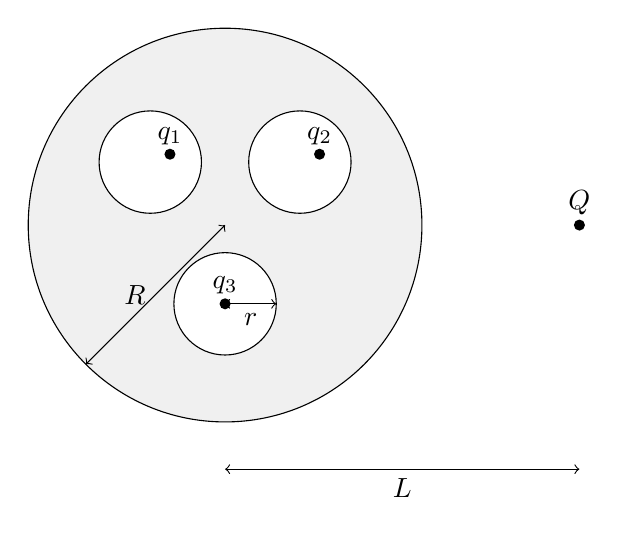
\begin{tikzpicture}

\fill[gray!12](0,0)circle(2.5);\draw(0,0)circle(2.5);
\foreach \x/\y/\n in {-.95/.8/1,.95/.8/2,0/-1/3}{\fill[white](\x,\y)circle(.65);\draw(\x,\y)circle(.65);}
\fill(-.7,.9)circle(2pt)node[above]{$q_1$};\fill(1.2,.9)circle(2pt)node[above]{$q_2$};\fill(0,-1)circle(2pt)node[above]{$q_3$};
\draw[<->](0,-1)--(.65,-1)node[midway,below]{$r$};\draw[<->](0,0)--(-1.768,-1.768)node[midway,left]{$R$};
\fill(4.5,0)circle(2pt)node[above]{$Q$};\draw[<->](0,-3.1)--(4.5,-3.1)node[midway,below]{$L$};

\end{tikzpicture}}
\end{question}
\begin{solution}\textbf{逐腔用高斯面求内壁与外表面总量}\par\nobreak
在 图\ref{fig:e3:example:10:s} 各腔外、金属内分别取高斯面，三个内壁总量依次为 $-q_i$。导体总量零，故外表面总量 $S=q_1+q_2+q_3$。从外部看，球面等势、净量 $S$；用孤立球像解，中心补充像为 $S+QR/L$，所以
\[
 V_C=kS/R+kQ/L.
\]


\par\medskip\Needspace{4\baselineskip}\noindent\textbf{从共同金属电势分离第三腔的反作用势}\par\nobreak
第三腔中心电荷使该腔内壁均匀带 $-q_3$，其中心电势贡献为 $-kq_3/r$，其他导体部分在腔内只贡献常数。因此中心除自场外电势是 $V_C-kq_3/r$。
\typeout{ECFIG:fig:e3:example:10:p}\fig{fig:e3:example:10:p}{逐腔高斯面确定内壁总量；第三腔中心充电时外表面总量与共同电势随 $\xi$ 改变}{\begin{tikzpicture}

\fill[gray!12](0,0)circle(2.5);\draw(0,0)circle(2.5);
\foreach \x/\y/\n in {-.95/.8/1,.95/.8/2,0/-1/3}{\fill[white](\x,\y)circle(.65);\draw(\x,\y)circle(.65);\draw[guide](\x,\y)circle(.8);}
\fill(-.7,.9)circle(2pt)node[above]{$q_1$};\fill(1.2,.9)circle(2pt)node[above]{$q_2$};\fill(0,-1)circle(2pt)node[above]{$\xi$};
\node at(-1,.45){$-q_1$};\node at(.95,.45){$-q_2$};\node at(0,-1.45){$-\xi$};
\fill(4.5,0)circle(2pt)node[above]{$Q$};\draw[guide](2.3,1)--(3,2.3)node[right]{$S=q_1+q_2+\xi$};
\node at(3.7,-2){第三腔：$V_{\text{反}}=V_C-k\xi/r$};

\end{tikzpicture}}



\par\medskip\Needspace{4\baselineskip}\noindent\textbf{在充电中间态积分，区分固定项与自诱导项}\par\nobreak
图\ref{fig:e3:example:10:p} 将中心电量从 $0$ 增至 $q_3$ 的中间值 $\xi$ 时，反作用电势为
\[
 V_{\text{反}}(\xi)=k\left[\frac{q_1+q_2}{R}+\frac QL\right]
 +k\xi\left(\frac1R-\frac1r\right).
\]
故建立电荷的外功为
\[
 \begin{aligned}
 W&=\int_0^{q_3}V_{\text{反}}(\xi)\dd\xi\\
 &=k\left[\frac{q_1+q_2}{R}+\frac QL\right][\xi]_0^{q_3}
 +k\left(\frac1R-\frac1r\right)\left[\frac{\xi^2}{2}\right]_0^{q_3}\\
 &=kq_3\left[\frac{q_1+q_2}{R}+\frac QL\right]
 +\frac{kq_3^2}2\left(\frac1R-\frac1r\right).
\end{aligned}
\]
这里明确采用逐渐充电的功；用最终电量乘最终反作用电势，会把由自身引起的感应项多算一倍。



\par\medskip\Needspace{4\baselineskip}\noindent\textbf{按新的外表面总量重建各区域分布}\par\nobreak
移走前两电荷后，两空腔零场，内壁密度零；第三腔内壁仍为 $-q_3/(4\pi r^2)$。外表面净量变为 $q_3$。令 $\theta$ 从指向 $Q$ 的轴量起，其面密度为
\[
 \sigma_{\text{外}}(\theta)=\frac{q_3+QR/L}{4\pi R^2}
 -\frac{Q(L^2-R^2)}{4\pi R(L^2+R^2-2LR\cos\theta)^{3/2}}.
\]
外部 $Q$ 改变外表面分布与共同电势，却不改变中心电荷在第三腔产生的球对称场。\end{solution}
\begin{question}\begin{example}[薄金属圆盘的近轴感应]\label{e3:example:11}
半径 $R$ 的薄金属圆盘，轴线上距盘 $a\ll R$ 处有点电荷 $q$。先接地，再讨论孤立圆盘净量为 $Q$。求接地总感应电荷及盘中心附近两面的电荷密度，说明局部近似范围。
无外电荷时，圆盘电势为 $V_0$ 的轴线势已知为
$\phi(z)=2V_0\arctan(R/|z|)/\pi$；净电荷为 $Q_0$ 的自由圆盘，距轴 $s<R$ 处每一面的平衡密度已知为
$\sigma_0(s)=Q_0/[4\pi R\sqrt{R^2-s^2}]$。
\end{example}
\typeout{ECFIG:fig:e3:example:11:s}\fig{fig:e3:example:11:s}{题设：薄金属圆盘的近轴感应}{\begin{tikzpicture}[scale=.88]
\draw[world](0,0)ellipse(2 and .45);\draw(2,0)--(3,0)to[nos](3,-1.5)node[ground]{};\draw[guide](0,-.6)--(0,2.7);\fill(0,1.9)circle(2pt)node[right]{$q$};\draw[dim](.65,0)--(.65,1.9)node[midway,right]{$a$};\draw[dim](0,-.9)--(2,-.9)node[midway,below]{$R$};
\end{tikzpicture}}
\end{question}
\begin{solution}\textbf{用互易关系先求有限盘的接地总感应量}\par\nobreak
图\ref{fig:e3:example:11:s} 中先比较无外电荷而盘电势为 $V_0$ 的状态，和有外点电荷、盘接地的状态。互易关系给
\[
 Q_gV_0+q\phi(a)=0,\qquad
 Q_g=-\frac{2q}{\pi}\arctan\frac Ra.
\]
当 $a/R\to0$，$Q_g\to-q$。这给出了有限圆盘的总量；局部平面近似本身不能给出有限尺寸修正。
\typeout{ECFIG:fig:e3:example:11:p}\fig{fig:e3:example:11:p}{左图为接地时的近轴局部感应，右图为另加净量的自由盘分布，两面均须积分}{\begin{tikzpicture}

\begin{scope}
\draw[thick](-2.5,0)--(2.5,0);\draw(2.5,0)--(3,0)--(3,-1)node[ground]{};\fill(0,1.7)circle(2pt)node[above]{$q$};\draw[<->](.8,0)--(.8,1.7)node[midway,right]{$a$};
\foreach \x in {-.8,-.4,0,.4,.8}{\node[blue]at(\x,-.3){$-$};}\node at(0,-1.2){上侧主项 $\sigma_{g,+}$};\node at(0,-2){下侧局部主项近零};
\end{scope}
\begin{scope}[xshift=7.5cm]
\draw[thick](-2.5,0)--(2.5,0);\foreach \x in {-2.3,-1.9,-1.1,0,1.1,1.9,2.3}{\node[red]at(\x,.35){$+$};\node[red]at(\x,-.35){$+$};}
\node at(0,1.5){示意 $\Delta Q>0$};\node at(0,-1.2){两面各有 $\sigma_{\text{加}}(s)$};\node at(0,-2){近边缘密度增强};
\end{scope}

\end{tikzpicture}}



\par\medskip\Needspace{4\baselineskip}\noindent\textbf{只在近轴局部使用平面感应主项}\par\nobreak
图\ref{fig:e3:example:11:p}左图在距轴 $s\ll R$ 且 $a\ll R$ 的上侧，接地面密度的主要项是
\[
 \sigma_{g,+}(s)\simeq-\frac{qa}{2\pi(s^2+a^2)^{3/2}},
\]
下侧局部主要项近于零。

\par\medskip\Needspace{4\baselineskip}\noindent\textbf{叠加自由盘解补足指定净量}\par\nobreak
接地解使整个圆盘为零势；孤立后仍须使整个盘面等势，只是常数势不再限定为零。
在线性静电问题中，叠加一个无外电荷的自由圆盘解，只会给盘面增加常数势，
不会改变外点电荷 $q$。取附加净量为 $\Delta Q=Q-Q_g$，总净量便回到题设的 $Q$。
使用题给自由盘的平衡密度，将 $Q_0$ 换成 $\Delta Q$，得到每一面
\[
 \sigma_{\text{加}}(s)=\frac{\Delta Q}{4\pi R\sqrt{R^2-s^2}}.
\]


\par\medskip\Needspace{4\baselineskip}\noindent\textbf{核对两面的电量积分}\par\nobreak
代入每一面的面密度，先保留两个面的因子：
\[
 Q_{\text{加}}=2\int_0^R2\pi s\sigma_{\text{加}}\,\dd s
 =\frac{\Delta Q}{R}\int_0^R\frac{s\,\dd s}{\sqrt{R^2-s^2}}.
\]
令 $z=R^2-s^2$，则 $\dd z=-2s\,\dd s$；$s=0,R$ 对应 $z=R^2,0$。
于是
\[
 \int_0^R\frac{s\,\dd s}{\sqrt{R^2-s^2}}
 =-\frac12\int_{R^2}^{0}z^{-1/2}\dd z
 =-\bigl[\sqrt z\bigr]_{R^2}^{0}=R,
 \qquad Q_{\text{加}}=\Delta Q.
\]
边缘的密度虽发散，这个反常积分的极限有限。
图\ref{fig:e3:example:11:p}右图的上下两面必须同时计入。
这个积分只检查归一化；盘面等势的依据是题给的自由圆盘平衡解，不能由总电量正确反推任意分布都能保持等势。


\par\medskip\Needspace{4\baselineskip}\noindent\textbf{展开局部密度并标明消项和边缘限制}\par\nobreak
先说明有限尺寸与近轴展开的两个小参数。令$\eta=a/R>0$，用$\arctan(R/a)=\pi/2-\arctan\eta$改写总感应量。函数$G(\eta)=\arctan\eta$满足
\[
G'(\eta)=\frac1{1+\eta^2},\qquad
G''(\eta)=-\frac{2\eta}{(1+\eta^2)^2}.
\]
由$G(0)=0$、$G'(0)=1$、$G''(0)=0$，零点附近$G(\eta)=\eta+O(\eta^3)$，因而$Q_g=-q+(2q/\pi)\eta+O(q\eta^3)$，附加净量的主项才是$\Delta Q=Q-Q_g\simeq Q+q$。

另令$z=s^2/R^2$。自由盘密度中的几何因子为$1/[R\sqrt{R^2-s^2}]=R^{-2}(1-z)^{-1/2}$。对$H(z)=(1-z)^{-1/2}$用链式法则，$H'(z)=(-1/2)(1-z)^{-3/2}(-1)=\tfrac12(1-z)^{-3/2}$，所以$H(0)=1$、$H'(0)=1/2$，故
\[
\sigma_{\text{加}}(s)=\frac{\Delta Q}{4\pi R^2}
\left[1+\frac{s^2}{2R^2}+O\!\left(\frac{s^4}{R^4}\right)\right].
\]
同时只保留$\eta$和$z$的主项，再叠加接地局部解，得到中心附近
\[
 \sigma_+(s)\simeq-\frac{qa}{2\pi(s^2+a^2)^{3/2}}
 +\frac{Q+q}{4\pi R^2},\qquad
 \sigma_-(s)\simeq\frac{Q+q}{4\pi R^2}.
\]
这里把 $Q_g$ 的主项取为 $-q$，且忽略 $s^2/R^2$。若 $Q+q$ 的主项恰抵消，应继续保留 $Q_g$ 的有限尺寸修正及接地盘局部分布的高阶项，不能据主项为零断言下表面精确无电。

接近盘边缘时这组局部表达式失效，附加密度本身还具有边缘增强，不能写成整个盘面处处均匀。近轴吸引力主要项为 $kq^2/(4a^2)$；孤立盘附加净量对力的修正，要与盘的完整外场结合后再计算。\end{solution}
\begin{question}\begin{example}[内球接地而外壳附近有点电荷]\label{e3:example:12}
同心薄金属球壳半径 $R_A<R_B$，内壳接地、外壳原中性且孤立。外点电荷 $q$ 距球心 $d>R_B$。求内球感应净量及外壳电势。忽略地线小孔的漏场。
\end{example}
\typeout{ECFIG:fig:e3:example:12:s}\fig{fig:e3:example:12:s}{内球地线穿过外壳的绝缘小孔，外壳保持孤立；半径 $R_A,R_B$ 分别标明}{\begin{tikzpicture}

\draw(0,0)circle(.8);\draw(0,0)circle(2);\fill[white](-.18,-2.2)rectangle(.18,-1.8);\draw(-.18,-2.2)rectangle(.18,-1.8);
\draw(0,-.8)--(0,-3.2)node[ground]{};\fill(0,0)circle(1.5pt)node[below right]{$O$};
\draw[<->](0,0)--(-.566,.566)node[midway,left]{$R_A$};\draw[<->](0,0)--(1,1.732)node[midway,right]{$R_B$};
\fill(4.2,0)circle(2pt)node[above]{$q$};\draw[<->](0,-3.9)--(4.2,-3.9)node[midway,below]{$d$};\draw[guide](.18,-2)--(2,-2.8)node[right]{绝缘孔};

\end{tikzpicture}}
\end{question}
\begin{solution}\textbf{用外壳中性条件建立三个表面总量}\par\nobreak
图\ref{fig:e3:example:12:s} 中令内球取得净量 $Q_A$。外壳内表面为 $-Q_A$，外表面为 $Q_A$，外壳净量仍零。外区域等效于净量 $Q_A$ 的等势球壳受外点电荷作用，故壳电势
$V_B=kQ_A/R_B+kq/d$。
\typeout{ECFIG:fig:e3:example:12:p}\fig{fig:e3:example:12:p}{内球接地而外壳净量为零；外壳两个表面的总量相反，腔内球对称场由 $Q_A$ 决定}{\begin{tikzpicture}

\draw(0,0)circle(.8);\draw(0,0)circle(2);\fill[white](-.18,-2.2)rectangle(.18,-1.8);\draw(-.18,-2.2)rectangle(.18,-1.8);\draw(0,-.8)--(0,-3.2)node[ground]{};
\node at(0,.2){$Q_A$};\draw[guide](-1.8,.5)--(-3,1.4)node[left]{内面 $-Q_A$};\draw[guide](1.8,.5)--(3,1.5)node[right]{外面 $+Q_A$};
\fill(4.5,0)circle(2pt)node[above]{$q$};\node at(3.7,-1.3){$V_B=kQ_A/R_B+kq/d$};\node at(-3,-1.5){$V_A=0$};

\end{tikzpicture}}



\par\medskip\Needspace{4\baselineskip}\noindent\textbf{将内球接地条件与间隙电势差联立}\par\nobreak
图\ref{fig:e3:example:12:p} 内外球间没有别的电荷，球对称场使 $V_A-V_B=kQ_A(1/R_A-1/R_B)$。内球接地 $V_A=0$，联立得
\[
 0=\frac{kQ_A}{R_A}+\frac{kq}{d},\qquad
 Q_A=-\frac{qR_A}{d},\quad
 V_B=\frac{kq}{d}\left(1-\frac{R_A}{R_B}\right).
\]


\par\medskip\Needspace{4\baselineskip}\noindent\textbf{解释外部共同电势如何引起接地内球电荷变化}\par\nobreak
外点电荷的作用通过外壳共同电势进入，不能把腔内无外场误解为内球电荷不受外电荷影响。接地内球可通过地线交换电荷，改变的是腔内球对称场的幅度。\end{solution}
\begin{question}\begin{example}[金属球与轴线上均匀带电环]\label{e3:example:13}
金属球半径 $R$，球心到均匀带电细环圆心的轴向距离为 $a>R$，环半径 $b$、总量 $q$，各点到球心等距 $D=\sqrt{a^2+b^2}$。求球接地、孤立中性、保持电势 $U$ 时的净量与电势；比较保持 $U$ 和接地时环受力的改变量。
\end{example}
\typeout{ECFIG:fig:e3:example:13:s}\fig{fig:e3:example:13:s}{球心位于圆环轴线上；轴向距离为 $a$，环点到球心的等距为 $D$}{\begin{tikzpicture}

\draw(0,0)circle(1.5);\fill(0,0)circle(1.5pt)node[below left]{$O$};\draw[<->](0,0)--(-1.06,1.06)node[midway,left]{$R$};
\draw(3.5,0)ellipse(.3 and 1.1);\fill(3.5,1.1)circle(1.7pt);\draw[guide](0,0)--(3.5,1.1)node[midway,above]{$D$};
\draw[<->](3.5,0)--(3.5,1.1)node[midway,right]{$b$};\draw[<->](0,-2.2)--(3.5,-2.2)node[midway,below]{$a$};\node at(4.5,-.8){环总量 $q$};

\end{tikzpicture}}
\end{question}
\begin{solution}\textbf{对环的每个等距微元叠加接地球像量}\par\nobreak
把 图\ref{fig:e3:example:13:s} 的环分为微元 $\dd q$，每个微元都距球心 $D$。接地球对该微元的像量是$-R\,\dd q/D$。由于$R/D$在整环上不变，对所有微元求和：
\[
Q_g=\oint_{\text{环}}-\frac{R}{D}\,\dd q
=-\frac{R}{D}\oint_{\text{环}}\dd q
=-\frac{qR}{D}.
\]
这里$\oint_{\text{环}}\dd q=q$就是整环的总电荷；球面电势由每对真实微元与像微元分别抵消，故总球电势仍为零。
\typeout{ECFIG:fig:e3:example:13:p}\fig{fig:e3:example:13:p}{等距环经球面反演形成像环；增加中心像只改变球面共同电势及环的轴向受力}{\begin{tikzpicture}

\draw(0,0)circle(1.5);\draw(3.5,0)ellipse(.3 and 1.1);\draw[blue,dashed](.585067,0)ellipse(.06 and .183878);
\fill(3.5,1.1)circle(2pt)node[above]{$\dd q$};\draw[guide](0,0)--(3.5,1.1)node[midway,above]{$D$};\fill[blue](.585067,.183878)circle(1.5pt);
\draw[blue,dashed](0,0)circle(.1);\node[blue,below left]at(0,0){$q_0$};\draw[guide](.585067,-.2)--(1.5,-1.8)node[right]{像环总量 $-qR/D$};
\draw[force](3.5,0)--(5,0)node[right]{$\Delta F_a$};\node at(0,2.3){球半径 $R$};\node at(3.5,2.3){环半径 $b$};
\draw[<->](0,-2.6)--(3.5,-2.6)node[midway,below]{$a$};

\end{tikzpicture}}



\par\medskip\Needspace{4\baselineskip}\noindent\textbf{分别按零净量和指定电势补中心像}\par\nobreak
图\ref{fig:e3:example:13:p} 孤立中性球需补中心像 $q_0=qR/D$，所以净量零、球电势 $V=kq/D$。指定球电势为 $U$ 时，补中心像 $q_0=RU/k$，球净量
\[
 Q_U=\frac{RU}{k}-\frac{qR}{D}.
\]


\par\medskip\Needspace{4\baselineskip}\noindent\textbf{只对新增中心像的力作轴向投影}\par\nobreak
由接地改成电势 $U$，偏心像分布保持，只增加中心像 $RU/k$。环每微元因中心像增加的力沿球心到该微元方向，其轴向分量积分为
\[
 \Delta F_a=\int\frac{k(RU/k)\,\dd q}{D^2}\frac aD
 =\frac{qRUa}{(a^2+b^2)^{3/2}}.
\]


\par\medskip\Needspace{4\baselineskip}\noindent\textbf{检查力的改变量与原感应力的区别}\par\nobreak
向远离球心取正。$qU>0$ 时斥力增加，$qU<0$ 时吸引增加；这求的是力的改变量，不等于环原有的全部感应力。\end{solution}
